%2multibyte Version: 5.50.0.2960 CodePage: 65001
% !TeX root = ./Slides_Lez_03_Valori_Attesi_Condizionati_verCLA.tex
%******************
% Macro matematiche ufficiali del progetto MQF
% Coerenti con MQF_Notazione.tex
%******************
% Fallback utile per compilazione esterna se qualche titolo resta scritto come \QTR.
% Scientific WorkPlace usa \QTR internamente; in Beamer \QTR{frametitle}{Titolo}
% deve espandersi in \frametitle{Titolo}.

\documentclass[handout]{beamer}%
\usepackage{mathpazo}
%\usepackage{hyperref}
\usepackage{multimedia}
\usepackage{amsmath}
\usepackage{amsfonts}
\usepackage{amssymb}
\usepackage{graphicx}%
\setcounter{MaxMatrixCols}{30}
%TCIDATA{OutputFilter=latex2.dll}
%TCIDATA{Version=5.50.0.2960}
%TCIDATA{Codepage=65001}
%TCIDATA{CSTFile=beamer.cst}
%TCIDATA{Created=Saturday, May 16, 2026 09:09:59}
%TCIDATA{LastRevised=Saturday, October 17, 2026 21:30:00}
%TCIDATA{<META NAME="GraphicsSave" CONTENT="32">}
%TCIDATA{<META NAME="SaveForMode" CONTENT="2">}
%TCIDATA{BibliographyScheme=Manual}
%TCIDATA{<META NAME="DocumentShell" CONTENT="Other Documents\SW\Slides - Beamer">}
%BeginMSIPreambleData
\graphicspath{{../graphics/}}
\providecommand{\U}[1]{\protect\rule{.1in}{.1in}}
%EndMSIPreambleData
\newenvironment{stepenumerate}{\begin{enumerate}[<+->]}{\end{enumerate}}
\newenvironment{stepitemize}{\begin{itemize}[<+->]}{\end{itemize} }
\newenvironment{stepenumeratewithalert}{\begin{enumerate}[<+-| alert@+>]}{\end{enumerate}}
\newenvironment{stepitemizewithalert}{\begin{itemize}[<+-| alert@+>]}{\end{itemize} }
\usetheme{Madrid}

\setbeamertemplate{footline}
{
  \leavevmode%
  \hbox{%
    \begin{beamercolorbox}[wd=.20\paperwidth,ht=2.25ex,dp=1ex,center]
      {author in head/foot}%
      \usebeamerfont{author in head/foot}\insertshortauthor
    \end{beamercolorbox}%
    \begin{beamercolorbox}[wd=.69\paperwidth,ht=2.25ex,dp=1ex,center]
      {title in head/foot}%
      \usebeamerfont{title in head/foot}\insertshorttitle
    \end{beamercolorbox}%
    \begin{beamercolorbox}[wd=.11\paperwidth,ht=2.25ex,dp=1ex,right]
      {date in head/foot}%
      \usebeamerfont{date in head/foot}%
      \insertshortdate{}\hspace*{2em}%
      \insertframenumber{} / \inserttotalframenumber\hspace*{2ex}
    \end{beamercolorbox}%
  }%
  \vskip0pt%
}

\providecommand{\R}{\mathbb{R}}
\providecommand{\N}{\mathbb{N}}
\providecommand{\E}{\mathbb{E}}
\providecommand{\Prob}{\mathbb{P}}
\providecommand{\Q}{\mathbb{Q}}
\providecommand{\F}{\mathcal{F}}
\providecommand{\B}{\mathcal{B}}
\providecommand{\G}{\mathcal{G}}
\providecommand{\1}{\mathbf{1}}
\providecommand{\Var}{\operatorname{Var}}
\providecommand{\Cov}{\operatorname{Cov}}
\providecommand{\VaR}{\operatorname{VaR}}
\providecommand{\CVaR}{\operatorname{CVaR}}
\providecommand{\argmin}{\operatorname*{arg\,min}}
\providecommand{\argmax}{\operatorname*{arg\,max}}
\providecommand{\EVPI}{\operatorname{EVPI}}
\providecommand{\VSS}{\operatorname{VSS}}
\providecommand{\QTR}[2]{\csname #1\endcsname{#2}}
%BeginMSIPreambleData
\ifx\pdfoutput\relax\let\pdfoutput=\undefined\fi
\newcount\msipdfoutput
\ifx\pdfoutput\undefined\else
\ifcase\pdfoutput\else
\msipdfoutput=1
\ifx\paperwidth\undefined\else
\ifdim\paperheight=0pt\relax\else\pdfpageheight\paperheight\fi
\ifdim\paperwidth=0pt\relax\else\pdfpagewidth\paperwidth\fi
\fi\fi\fi
%EndMSIPreambleData


\title[Lez. 3 - Valori attesi condizionati e informazione]{Lezione 3 - Valori attesi condizionati e informazione}
\subtitle{Metodi Quantitativi per la Finanza}
\author[P. Falbo, C. Pelizzari]{{\LARGE Paolo Falbo, Cristian Pelizzari}}
\institute[]{{\large Dipartimento di Economia e Management}}
\date[]{}
\titlegraphic{

\includegraphics[height=1.25cm]{../graphics/MQF_logo.png}\hspace{0.8cm}%

\includegraphics[height=1.25cm]{../graphics/logo-Unibs-esteso.png}
}

\begin{document}
\maketitle

%******************
% BLOCCO: Apertura
%******************
\section{Apertura}

\subsection{Domanda guida}
%TCIMACRO{\TeXButton{BeginFrame}{\begin{frame}}}%
%BeginExpansion
\begin{frame}%
%EndExpansion

\QTR{frametitle}{Valori attesi condizionati e informazione}

%TCIMACRO{\TeXButton{Transparency}{\setbeamercovered{transparent=20}}}%
%BeginExpansion
\setbeamercovered{transparent=20}%
%EndExpansion

\begin{center}
{\Large Come cambia la valutazione di un payoff quando arriva nuova
informazione?}
\end{center}

\medskip

In finanza, una valutazione non dipende solo dal payoff futuro, ma anche
dall'informazione disponibile al momento della decisione:

\medskip

\begin{stepitemize}
\item senza informazione aggiuntiva si valuta una media non condizionata,
$\E[H]$;

\item osservando un evento rilevante cambiano gli scenari compatibili e i
loro pesi, $\E[H\mid A]$;

\item prima di osservare un segnale, la valutazione dipende da ci\`{o} che il
segnale riveler\`{a}, $\E[H\mid\G]$.
\end{stepitemize}

%TCIMACRO{\TeXButton{Transition: Box Out}{\transboxout}}%
%BeginExpansion
\transboxout%
%EndExpansion
%TCIMACRO{\TeXButton{EndFrame}{\end{frame}}}%
%BeginExpansion
\end{frame}%
%EndExpansion
%*********************************************

\subsection{Motivazione finanziaria}
%TCIMACRO{\TeXButton{BeginFrame}{\begin{frame}}}%
%BeginExpansion
\begin{frame}%
%EndExpansion

\QTR{frametitle}{Valutare prima che l'incertezza sia risolta}

%TCIMACRO{\TeXButton{Transparency}{\setbeamercovered{transparent=20}}}%
%BeginExpansion
\setbeamercovered{transparent=20}%
%EndExpansion

Molte grandezze finanziarie sono valutate prima che l'incertezza sia
risolta.

\medskip

\begin{stepitemize}
\item Un \textbf{payoff} futuro $H$ dipende dallo stato di mercato che si
realizzer\`{a}.

\item Una \textbf{perdita} futura $L$ dipende da prezzi, tassi, default e
fattori di rischio non ancora osservati.

\item La valutazione iniziale usa l'informazione disponibile oggi:
\[
\E[H], \qquad \E[L].
\]

\item Se arriva nuova informazione, la valutazione deve essere aggiornata:
\[
\E[H\mid \G], \qquad \E[L\mid \G].
\]
\end{stepitemize}

%TCIMACRO{\TeXButton{Transition: Box Out}{\transboxout}}%
%BeginExpansion
\transboxout%
%EndExpansion
%TCIMACRO{\TeXButton{EndFrame}{\end{frame}}}%
%BeginExpansion
\end{frame}%
%EndExpansion
%*********************************************

\subsection{Un esempio che contiene la lezione}
%TCIMACRO{\TeXButton{BeginFrame}{\begin{frame}}}%
%BeginExpansion
\begin{frame}%
%EndExpansion

\QTR{frametitle}{Un esempio che contiene l'intera lezione}

%TCIMACRO{\TeXButton{Transparency}{\setbeamercovered{transparent=20}}}%
%BeginExpansion
\setbeamercovered{transparent=20}%
%EndExpansion

Un payoff terminale $H$ su quattro scenari macro-finanziari:

\begin{center}
{\small
\begin{tabular}{c|l|c|c}
$\omega$ & Scenario & $\Prob(\{\omega\})$ & $H(\omega)$ \\ \hline
$\omega_1$ & espansione & $0.25$ & $120$ \\
$\omega_2$ & crescita moderata & $0.35$ & $105$ \\
$\omega_3$ & stagnazione & $0.25$ & $90$ \\
$\omega_4$ & recessione & $0.15$ & $60$
\end{tabular}
}
\end{center}

\[
\E[H]=0.25\cdot120+0.35\cdot105+0.25\cdot90+0.15\cdot60=98.25.
\]

Prima della scadenza arriva un segnale macroeconomico: favorevole,
$A=\{\omega_1,\omega_2\}$, oppure sfavorevole, $A^c=\{\omega_3,\omega_4\}$.
\[
\E[H\mid A]=\frac{0.25\cdot120+0.35\cdot105}{0.60}=111.25,
\]
\[
\E[H\mid A^c]=\frac{0.25\cdot90+0.15\cdot60}{0.40}=78.75.
\]

%TCIMACRO{\TeXButton{Transition: Box Out}{\transboxout}}%
%BeginExpansion
\transboxout%
%EndExpansion
%TCIMACRO{\TeXButton{EndFrame}{\end{frame}}}%
%BeginExpansion
\end{frame}%
%EndExpansion
%*********************************************

%TCIMACRO{\TeXButton{BeginFrame}{\begin{frame}}}%
%BeginExpansion
\begin{frame}%
%EndExpansion

\QTR{frametitle}{Nell'esempio ci sono gi\`{a} tre valutazioni}

%TCIMACRO{\TeXButton{Transparency}{\setbeamercovered{transparent=20}}}%
%BeginExpansion
\setbeamercovered{transparent=20}%
%EndExpansion

\begin{stepenumerate}
\item [1.] \textbf{Prima del segnale}: $\E[H]=98.25$, un \textbf{numero}.

\item [2.] \textbf{Dopo aver osservato il segnale}: $\E[H\mid A]=111.25$
oppure $\E[H\mid A^c]=78.75$, un \textbf{numero}.

\item [3.] \textbf{Prima di osservarlo, sapendo che arriver\`{a}}: con
$\G=\sigma(A,A^c)$, una \textbf{variabile casuale}
\[
\E[H\mid\G]=111.25\,\1_{A}+78.75\,\1_{A^c}.
\]
\end{stepenumerate}

\medskip

Le tre valutazioni sono fra loro \textbf{coerenti}:
\[
98.25=111.25\cdot0.60+78.75\cdot0.40.
\]

\begin{center}
{\small La lezione sviluppa in generale questi tre passaggi e il legame che li
tiene insieme.}
\end{center}

%TCIMACRO{\TeXButton{Transition: Box Out}{\transboxout}}%
%BeginExpansion
\transboxout%
%EndExpansion
%TCIMACRO{\TeXButton{EndFrame}{\end{frame}}}%
%BeginExpansion
\end{frame}%
%EndExpansion
%*********************************************

\subsection{Percorso della lezione}
%TCIMACRO{\TeXButton{BeginFrame}{\begin{frame}}}%
%BeginExpansion
\begin{frame}%
%EndExpansion

\QTR{frametitle}{Percorso della lezione: la scala dell'informazione}

%TCIMACRO{\TeXButton{Transparency}{\setbeamercovered{transparent=20}}}%
%BeginExpansion
\setbeamercovered{transparent=20}%
%EndExpansion

Ogni gradino aggiunge informazione e cambia la natura della valutazione.

\medskip
\begin{center}
{\footnotesize
\begin{tabular}{c|l|c|l}
Gradino & Informazione & Valutazione & Natura \\ \hline
0 & nessuna & $\E[X]$ & numero \\
1 & un evento $A$ osservato & $\E[X\mid A]$ & numero \\
2 & un segnale da osservare, $\G$ & $\E[X\mid\G]$ & variabile casuale \\
3 & informazione nel tempo, $\F_t$ & $\E[H\mid\F_t]$ & previsione dinamica \\
\end{tabular}
}
\end{center}

\medskip

{\footnotesize
\textbf{Interpretazione:} $\E[X\mid\G]$ \`{e} la migliore previsione $\G$-misurabile.

\textbf{Coerenza:} valore atteso totale $\rightarrow$ $\E[\E[X\mid\G]]=\E[X]$ $\rightarrow$ propriet\`{a} della torre.

}

\begin{center}
{\small Due fili attraversano tutti i gradini: perch\'{e} si usa proprio la
media e perch\'{e} le valutazioni dei diversi gradini sono compatibili.}
\end{center}

%TCIMACRO{\TeXButton{Transition: Box Out}{\transboxout}}%
%BeginExpansion
\transboxout%
%EndExpansion
%TCIMACRO{\TeXButton{EndFrame}{\end{frame}}}%
%BeginExpansion
\end{frame}%
%EndExpansion
%*********************************************

\subsection{Obiettivi della lezione}
%TCIMACRO{\TeXButton{BeginFrame}{\begin{frame}}}%
%BeginExpansion
\begin{frame}%
%EndExpansion

\QTR{frametitle}{Obiettivi della lezione}

%TCIMACRO{\TeXButton{Transparency}{\setbeamercovered{transparent=20}}}%
%BeginExpansion
\setbeamercovered{transparent=20}%
%EndExpansion

Al termine della lezione, lo studente deve saper interpretare il valore
atteso condizionato come valutazione coerente con l'informazione disponibile.

\medskip

{\small
\begin{stepenumerate}
\item [1.] Calcolare $\E[X\mid A]$ nel caso discreto e continuo,
riconoscendolo come un numero.

\item [2.] Rappresentare l'informazione con partizioni e sigma-algebre e
costruire $\E[X\mid\G]$ come variabile casuale.

\item [3.] Interpretare $\E[X\mid\G]$ come migliore previsione
$\G$-misurabile.

\item [4.] Verificare la coerenza fra livelli informativi: valore atteso
totale e propriet\`{a} della torre.

\item [5.] Interpretare $\E[H\mid\F_t]$ come previsione al tempo $t$ di un
payoff terminale.

\item [6.] Applicare questi strumenti a payoff, perdite e scenari di stress.
\end{stepenumerate}
}

%TCIMACRO{\TeXButton{Transition: Box Out}{\transboxout}}%
%BeginExpansion
\transboxout%
%EndExpansion
%TCIMACRO{\TeXButton{EndFrame}{\end{frame}}}%
%BeginExpansion
\end{frame}%
%EndExpansion
%*********************************************

%******************
% BLOCCO: Gradino 1: un evento osservato
%******************
\section{Gradino 1: un evento osservato}

\subsection{Dove siamo: gradino 1}
%TCIMACRO{\TeXButton{BeginFrame}{\begin{frame}}}%
%BeginExpansion
\begin{frame}%
%EndExpansion

\QTR{frametitle}{Dove siamo: gradino 1}

%TCIMACRO{\TeXButton{Transparency}{\setbeamercovered{transparent=20}}}%
%BeginExpansion
\setbeamercovered{transparent=20}%
%EndExpansion

\begin{center}
{\large Che cosa cambia se osservo un evento?}
\end{center}

\medskip

\begin{center}
{\footnotesize
\begin{tabular}{c|l|c|l}
Gradino & Informazione & Valutazione & Natura \\ \hline
0 & nessuna & $\E[X]$ & numero \\
\alert{1} & \alert{un evento $A$ osservato} & \alert{$\E[X\mid A]$} & \alert{numero} \\
2 & un segnale da osservare, $\G$ & $\E[X\mid\G]$ & variabile casuale \\
3 & informazione nel tempo, $\F_t$ & $\E[H\mid\F_t]$ & previsione dinamica \\
\end{tabular}
}
\end{center}

\medskip

{\footnotesize
\textbf{Interpretazione:} $\E[X\mid\G]$ \`{e} la migliore previsione $\G$-misurabile.

\textbf{Coerenza:} valore atteso totale $\rightarrow$ $\E[\E[X\mid\G]]=\E[X]$ $\rightarrow$ propriet\`{a} della torre.

}

%TCIMACRO{\TeXButton{Transition: Box Out}{\transboxout}}%
%BeginExpansion
\transboxout%
%EndExpansion
%TCIMACRO{\TeXButton{EndFrame}{\end{frame}}}%
%BeginExpansion
\end{frame}%
%EndExpansion
%*********************************************

\subsection{L'informazione cambia i pesi}
%TCIMACRO{\TeXButton{BeginFrame}{\begin{frame}}}%
%BeginExpansion
\begin{frame}%
%EndExpansion

\QTR{frametitle}{Osservare un evento cambia i pesi, non il payoff}

%TCIMACRO{\TeXButton{Transparency}{\setbeamercovered{transparent=20}}}%
%BeginExpansion
\setbeamercovered{transparent=20}%
%EndExpansion

Condizionare rispetto a un evento \textbf{non cambia} il payoff $H$:
cambiano gli scenari ritenuti compatibili con l'informazione osservata e
i pesi con cui essi vengono valutati.

\medskip

\begin{stepitemize}

\item Prima dell'informazione, ogni scenario $\omega\in\Omega$ contribuisce
secondo la probabilit\`{a} iniziale
\[
\Prob(\{\omega\}).
\]

\item Dopo l'osservazione di un evento $A$, restano rilevanti solo gli
scenari compatibili, $\omega\in A$, con pesi ricalcolati mediante le
\textbf{probabilit\`{a} condizionate}:
\[
\Prob(\{\omega\}\mid A)=\frac{\Prob(\{\omega\})}{\Prob(A)},
\qquad \omega\in A.
\]

\item Gli scenari fuori da $A$ ricevono probabilit\`{a} condizionata nulla.

\end{stepitemize}

%TCIMACRO{\TeXButton{Transition: Box Out}{\transboxout}}%
%BeginExpansion
\transboxout%
%EndExpansion
%TCIMACRO{\TeXButton{EndFrame}{\end{frame}}}%
%BeginExpansion
\end{frame}%
%EndExpansion
%*********************************************

\subsection{Valore atteso condizionato rispetto a un evento}
%TCIMACRO{\TeXButton{BeginFrame}{\begin{frame}}}%
%BeginExpansion
\begin{frame}%
%EndExpansion

\QTR{frametitle}{$\E[H\mid A]$: una media con i pesi condizionati}

%TCIMACRO{\TeXButton{Transparency}{\setbeamercovered{transparent=20}}}%
%BeginExpansion
\setbeamercovered{transparent=20}%
%EndExpansion

Sia $H$ una variabile casuale discreta integrabile e sia $A\in\F$ un evento con
$\Prob(A)>0$.

\medskip

\begin{stepitemize}
\item Il valore atteso condizionato rispetto ad $A$ \`{e}:
\[
\E[H\mid A]=\sum_h h\,\Prob(H=h\mid A).
\]

\item I pesi della media sono le \textbf{probabilit\`{a} condizionate}:
\[
\Prob(H=h\mid A)
=
\frac{\Prob(\{H=h\}\cap A)}{\Prob(A)}.
\]

\item L'evento $A$ seleziona l'informazione osservata; la media considera
solo gli esiti di $H$ coerenti con tale informazione.

\item $\E[H\mid A]$ \`{e} un \textbf{numero}: la valutazione media di
$H$ dopo aver osservato $A$.
\end{stepitemize}

%TCIMACRO{\TeXButton{Transition: Box Out}{\transboxout}}%
%BeginExpansion
\transboxout%
%EndExpansion
%TCIMACRO{\TeXButton{EndFrame}{\end{frame}}}%
%BeginExpansion
\end{frame}%
%EndExpansion
%*********************************************

\subsection{Formula con indicatrice}
%TCIMACRO{\TeXButton{BeginFrame}{\begin{frame}}}%
%BeginExpansion
\begin{frame}%
%EndExpansion

\QTR{frametitle}{Condizionare significa restringere e rinormalizzare}

%TCIMACRO{\TeXButton{Transparency}{\setbeamercovered{transparent=20}}}%
%BeginExpansion
\setbeamercovered{transparent=20}%
%EndExpansion

Sia $X$ una variabile casuale integrabile e sia $A\in\F$ con $\Prob(A)>0$:
\[
\E[X\mid A]
=
\frac{\E[X\1_{A}]}{\Prob(A)}.
\]

\begin{stepitemize}
\item $\1_{A}$ seleziona gli scenari in cui l'evento $A$ si verifica:
\textbf{restringere}.

\item $\E[X\1_{A}]$ somma il contributo di $X$ solo sugli scenari
compatibili con $A$.

\item La divisione per $\Prob(A)$ \textbf{rinormalizza} la media rispetto
alla probabilit\`{a} dell'evento condizionante.

\item Nell'esempio iniziale:
\[
\E[H\mid A]=\frac{0.25\cdot120+0.35\cdot105}{0.60}=\frac{66.75}{0.60}=111.25.
\]
\end{stepitemize}

%TCIMACRO{\TeXButton{Transition: Box Out}{\transboxout}}%
%BeginExpansion
\transboxout%
%EndExpansion
%TCIMACRO{\TeXButton{EndFrame}{\end{frame}}}%
%BeginExpansion
\end{frame}%
%EndExpansion
%*********************************************

\subsection{Caso continuo}
%TCIMACRO{\TeXButton{BeginFrame}{\begin{frame}}}%
%BeginExpansion
\begin{frame}%
%EndExpansion

\QTR{frametitle}{Nel caso continuo cambia la densit\`{a}}

%TCIMACRO{\TeXButton{Transparency}{\setbeamercovered{transparent=20}}}%
%BeginExpansion
\setbeamercovered{transparent=20}%
%EndExpansion

Il condizionamento modifica la \textbf{distribuzione} rispetto alla quale si
calcola la media:
\[
F_{X\mid A}(x)=\Prob(X\leq x\mid A).
\]

Se la distribuzione condizionata ammette densit\`{a} $f_{X\mid A}$, allora:
\[
\E[X\mid A]
=
\int_{-\infty}^{+\infty} x f_{X\mid A}(x)\,dx.
\]

\begin{stepitemize}
\item L'integrale \`{e} la stessa operazione di media, ma calcolata con i
\textbf{pesi condizionati}.

\item La grandezza $X$ non viene modificata: cambia la distribuzione
rilevante per la sua valutazione.
\end{stepitemize}

\begin{center}
{\small \textit{Prossimo passo: e se il segnale non \`{e} ancora stato osservato?}}
\end{center}

%TCIMACRO{\TeXButton{Transition: Box Out}{\transboxout}}%
%BeginExpansion
\transboxout%
%EndExpansion
%TCIMACRO{\TeXButton{EndFrame}{\end{frame}}}%
%BeginExpansion
\end{frame}%
%EndExpansion
%*********************************************

%******************
% BLOCCO: Gradino 2: un segnale ancora da osservare
%******************
\section{Gradino 2: un segnale ancora da osservare}

\subsection{Dove siamo: gradino 2}
%TCIMACRO{\TeXButton{BeginFrame}{\begin{frame}}}%
%BeginExpansion
\begin{frame}%
%EndExpansion

\QTR{frametitle}{Dove siamo: gradino 2}

%TCIMACRO{\TeXButton{Transparency}{\setbeamercovered{transparent=20}}}%
%BeginExpansion
\setbeamercovered{transparent=20}%
%EndExpansion

\begin{center}
{\large E se il segnale non l'ho ancora osservato?}
\end{center}

\medskip

\begin{center}
{\footnotesize
\begin{tabular}{c|l|c|l}
Gradino & Informazione & Valutazione & Natura \\ \hline
0 & nessuna & $\E[X]$ & numero \\
1 & un evento $A$ osservato & $\E[X\mid A]$ & numero \\
\alert{2} & \alert{un segnale da osservare, $\G$} & \alert{$\E[X\mid\G]$} & \alert{variabile casuale} \\
3 & informazione nel tempo, $\F_t$ & $\E[H\mid\F_t]$ & previsione dinamica \\
\end{tabular}
}
\end{center}

\medskip

{\footnotesize
\textbf{Interpretazione:} $\E[X\mid\G]$ \`{e} la migliore previsione $\G$-misurabile.

\textbf{Coerenza:} valore atteso totale $\rightarrow$ $\E[\E[X\mid\G]]=\E[X]$ $\rightarrow$ propriet\`{a} della torre.

}

%TCIMACRO{\TeXButton{Transition: Box Out}{\transboxout}}%
%BeginExpansion
\transboxout%
%EndExpansion
%TCIMACRO{\TeXButton{EndFrame}{\end{frame}}}%
%BeginExpansion
\end{frame}%
%EndExpansion
%*********************************************

\subsection{Partizioni informative}
%TCIMACRO{\TeXButton{BeginFrame}{\begin{frame}}}%
%BeginExpansion
\begin{frame}%
%EndExpansion

\QTR{frametitle}{Una partizione descrive ci\`{o} che il segnale potr\`{a} distinguere}

%TCIMACRO{\TeXButton{Transparency}{\setbeamercovered{transparent=20}}}%
%BeginExpansion
\setbeamercovered{transparent=20}%
%EndExpansion

Una \textbf{partizione informativa} descrive gli stati che diventano
distinguibili dopo l'osservazione di un segnale:
\[
\Omega = B_1\cup\cdots\cup B_n,
\qquad
B_i\cap B_j=\varnothing \quad \text{se } i\neq j.
\]

\begin{stepitemize}
\item Prima dell'osservazione non sappiamo quale blocco $B_i$ si
realizzer\`{a}.

\item Dopo l'osservazione sappiamo che lo scenario vero appartiene a uno
specifico blocco $B_i$.

\item Per ciascun blocco possiamo calcolare una \textbf{media locale}:
\[
\E[X\mid B_i].
\]

\item La partizione trasforma una sola valutazione globale in una famiglia
di valutazioni condizionate.
\end{stepitemize}

%TCIMACRO{\TeXButton{Transition: Box Out}{\transboxout}}%
%BeginExpansion
\transboxout%
%EndExpansion
%TCIMACRO{\TeXButton{EndFrame}{\end{frame}}}%
%BeginExpansion
\end{frame}%
%EndExpansion
%*********************************************

\subsection{Figura 3.1: partizione di Omega}
%TCIMACRO{\TeXButton{BeginFrame}{\begin{frame}}}%
%BeginExpansion
\begin{frame}%
%EndExpansion

\QTR{frametitle}{Una partizione raggruppa gli scenari indistinguibili}

%TCIMACRO{\TeXButton{Transparency}{\setbeamercovered{transparent=20}}}%
%BeginExpansion
\setbeamercovered{transparent=20}%
%EndExpansion

\begin{center}
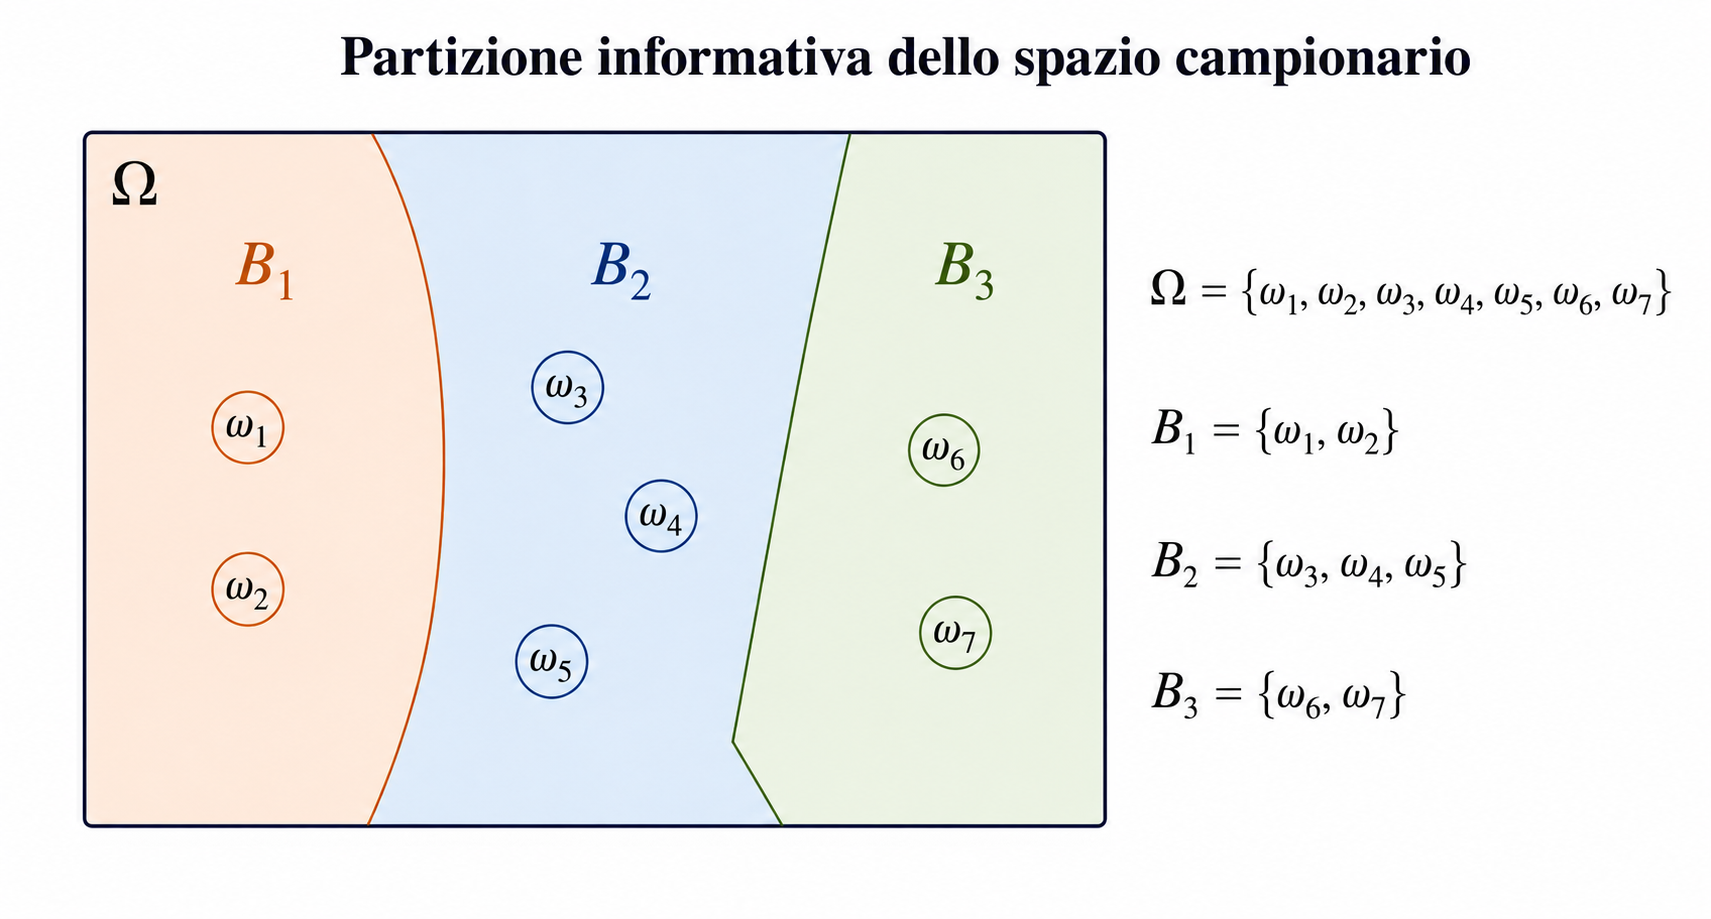
\includegraphics[width=0.72\textwidth]{../graphics/Cap03_Figura_3_1.png}
\end{center}

\begin{stepitemize}
\item Gli eventi $B_1,\ldots,B_n$ raccolgono scenari elementari non
distinguibili dalla stessa \textbf{informazione osservata}.

\item Osservare la partizione significa sapere quale evento $B_i$ si \`{e}
realizzato, senza necessariamente identificare il singolo scenario
elementare $\omega$.
\end{stepitemize}

%TCIMACRO{\TeXButton{Transition: Box Out}{\transboxout}}%
%BeginExpansion
\transboxout%
%EndExpansion
%TCIMACRO{\TeXButton{EndFrame}{\end{frame}}}%
%BeginExpansion
\end{frame}%
%EndExpansion
%*********************************************

\subsection{Valore atteso totale}
%TCIMACRO{\TeXButton{BeginFrame}{\begin{frame}}}%
%BeginExpansion
\begin{frame}%
%EndExpansion

\QTR{frametitle}{Prima del segnale: la media delle medie condizionate}

%TCIMACRO{\TeXButton{Transparency}{\setbeamercovered{transparent=20}}}%
%BeginExpansion
\setbeamercovered{transparent=20}%
%EndExpansion

\begin{center}
\fbox{\parbox{0.92\textwidth}{
\textbf{Coerenza (1/4) -- valore atteso totale.}
Se $\{B_1,\ldots,B_n\}$ \`{e} una partizione di $\Omega$ e $\Prob(B_i)>0$:
\[
\E[X]
=
\sum_{i=1}^{n}\E[X\mid B_i]\Prob(B_i).
\]
}}
\end{center}

\begin{stepitemize}
\item $\E[X\mid B_i]$ \`{e} la valutazione di $X$ quando l'informazione
osservata identifica il blocco $B_i$.

\item $\Prob(B_i)$ \`{e} il peso ex ante attribuito a quel possibile stato
informativo.

\item La media globale \`{e} una \textbf{media ponderata} delle valutazioni
condizionate. Nell'esempio iniziale:
\[
98.25=111.25\cdot0.60+78.75\cdot0.40.
\]
\end{stepitemize}

%TCIMACRO{\TeXButton{Transition: Box Out}{\transboxout}}%
%BeginExpansion
\transboxout%
%EndExpansion
%TCIMACRO{\TeXButton{EndFrame}{\end{frame}}}%
%BeginExpansion
\end{frame}%
%EndExpansion
%*********************************************

\subsection{Sigma-algebra generata e atomi}
%TCIMACRO{\TeXButton{BeginFrame}{\begin{frame}}}%
%BeginExpansion
\begin{frame}%
%EndExpansion

\QTR{frametitle}{La sigma-algebra generata descrive gli eventi osservabili}

%TCIMACRO{\TeXButton{Transparency}{\setbeamercovered{transparent=20}}}%
%BeginExpansion
\setbeamercovered{transparent=20}%
%EndExpansion

Data una partizione $\{B_1,\ldots,B_n\}$ di $\Omega$, l'informazione
osservabile \`{e} descritta dalla sigma-algebra
\[
\G=\sigma(B_1,\ldots,B_n).
\]

\begin{stepitemize}
\item Gli \textbf{atomi} di $\G$ sono gli eventi della partizione:
$B_1,\ldots,B_n$.

\item Gli \textbf{eventi osservabili} sono le unioni di atomi:
\[
B_{i_1}\cup\cdots\cup B_{i_k}.
\]

\item Un evento \`{e} osservabile rispetto a $\G$ se pu\`{o} essere
deciso conoscendo quale evento $B_i$ si \`{e} realizzato.

\item La sigma-algebra $\G$ formalizza quindi il contenuto informativo
della partizione.
\end{stepitemize}

%TCIMACRO{\TeXButton{Transition: Box Out}{\transboxout}}%
%BeginExpansion
\transboxout%
%EndExpansion
%TCIMACRO{\TeXButton{EndFrame}{\end{frame}}}%
%BeginExpansion
\end{frame}%
%EndExpansion
%*********************************************

\subsection{Figura 3.2: atomi ed eventi osservabili}
%TCIMACRO{\TeXButton{BeginFrame}{\begin{frame}}}%
%BeginExpansion
\begin{frame}%
%EndExpansion

\QTR{frametitle}{Atomi ed eventi osservabili}

%TCIMACRO{\TeXButton{Transparency}{\setbeamercovered{transparent=20}}}%
%BeginExpansion
\setbeamercovered{transparent=20}%
%EndExpansion

\begin{center}
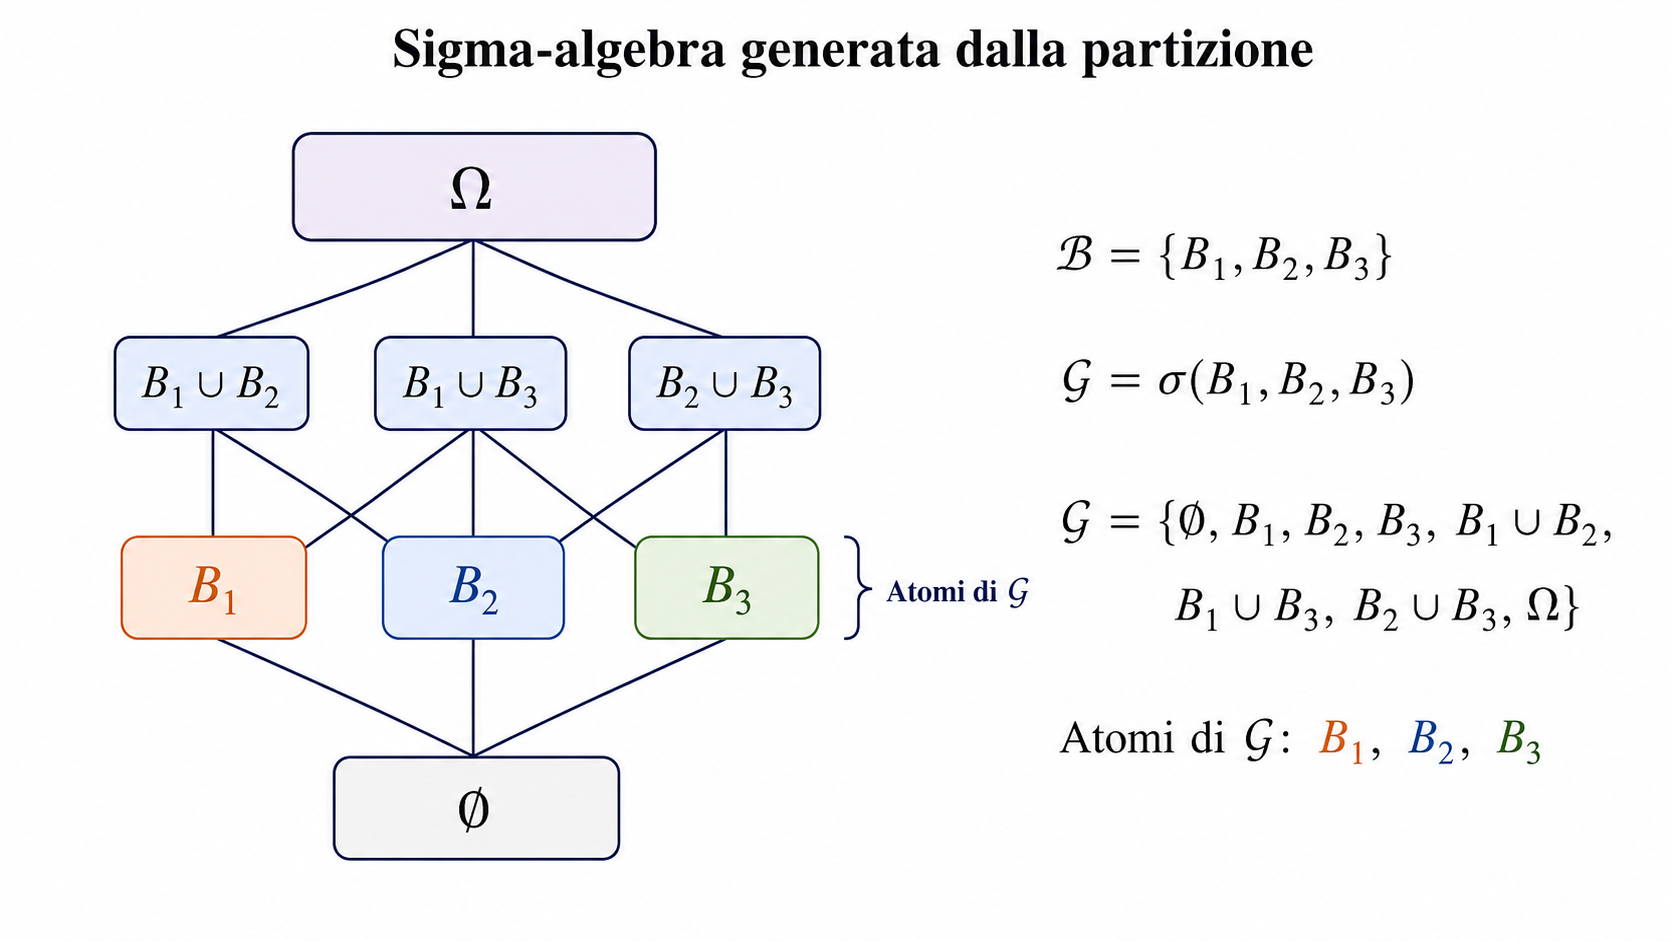
\includegraphics[width=0.80\textwidth]{../graphics/Cap03_Figura_3_2.png}
\end{center}

\begin{stepitemize}
\item Con la partizione $\{B_1,B_2,B_3\}$, la sigma-algebra
$\G=\sigma(B_1,B_2,B_3)$ contiene otto eventi: $\varnothing$, i tre atomi,
le loro unioni a due a due e $\Omega$.

\item I valori puntuali di una valutazione basata su $\G$ sono determinati
dagli atomi.
\end{stepitemize}

%TCIMACRO{\TeXButton{Transition: Box Out}{\transboxout}}%
%BeginExpansion
\transboxout%
%EndExpansion
%TCIMACRO{\TeXButton{EndFrame}{\end{frame}}}%
%BeginExpansion
\end{frame}%
%EndExpansion
%*********************************************

\subsection{E[X|G] come variabile casuale}
%TCIMACRO{\TeXButton{BeginFrame}{\begin{frame}}}%
%BeginExpansion
\begin{frame}%
%EndExpansion

\QTR{frametitle}{$\E[X\mid\G]$ \`{e} una variabile casuale}

%TCIMACRO{\TeXButton{Transparency}{\setbeamercovered{transparent=20}}}%
%BeginExpansion
\setbeamercovered{transparent=20}%
%EndExpansion

Se $X$ \`{e} integrabile, $\G=\sigma(B_1,\ldots,B_n)$ e
$\Prob(B_i)>0$ per ogni $i=1,\ldots,n$, il valore atteso condizionato
rispetto a $\G$ \`{e} la variabile casuale
\[
\E[X\mid\G]
=
\sum_{i=1}^{n}\E[X\mid B_i]\1_{B_i}.
\]

\begin{stepitemize}
\item Su ciascun atomo $B_i$, la variabile $\E[X\mid\G]$ \`{e}
\textbf{costante} e vale $\E[X\mid B_i]$.

\item Condizionare rispetto a un \textbf{evento} $A$ produce un
\textbf{numero}: $\E[X\mid A]$.

\item Condizionare rispetto a una \textbf{sigma-algebra} $\G$ produce una
\textbf{variabile casuale} osservabile rispetto a $\G$.
\end{stepitemize}

%TCIMACRO{\TeXButton{Transition: Box Out}{\transboxout}}%
%BeginExpansion
\transboxout%
%EndExpansion
%TCIMACRO{\TeXButton{EndFrame}{\end{frame}}}%
%BeginExpansion
\end{frame}%
%EndExpansion
%*********************************************

\subsection{Esempio con sette esiti elementari}
%TCIMACRO{\TeXButton{BeginFrame}{\begin{frame}}}%
%BeginExpansion
\begin{frame}%
%EndExpansion

\QTR{frametitle}{Esempio: $\E[H\mid\G]$ su sette scenari}

%TCIMACRO{\TeXButton{Transparency}{\setbeamercovered{transparent=20}}}%
%BeginExpansion
\setbeamercovered{transparent=20}%
%EndExpansion

Sia $\Omega=\{\omega_1,\ldots,\omega_7\}$ e sia
$\G=\sigma(B_1,B_2,B_3)$, con
\[
B_1=\{\omega_1,\omega_2\},\quad
B_2=\{\omega_3,\omega_4,\omega_5\},\quad
B_3=\{\omega_6,\omega_7\}.
\]

\begin{center}
{\scriptsize
\begin{tabular}{c|c|c|c}
Evento della partizione & Probabilit\`{a} & Valori di $H$ &
Media condizionata \\ \hline
$B_1$ & $0.10,\ 0.15$ & $130,\ 110$ &
$\E[H\mid B_1]=118$ \\
$B_2$ & $0.15,\ 0.20,\ 0.10$ & $100,\ 90,\ 80$ &
$\E[H\mid B_2]=91.111$ \\
$B_3$ & $0.18,\ 0.12$ & $70,\ 50$ &
$\E[H\mid B_3]=62$
\end{tabular}
}
\end{center}

\medskip

Prima del segnale la valutazione \`{e} il numero $\E[H]=89.10$. Rispetto a
$\G$ la valutazione \`{e} la variabile casuale
\[
\E[H\mid\G]
=
118\,\1_{B_1}
+
91.111\,\1_{B_2}
+
62\,\1_{B_3}.
\]

%TCIMACRO{\TeXButton{Transition: Box Out}{\transboxout}}%
%BeginExpansion
\transboxout%
%EndExpansion
%TCIMACRO{\TeXButton{EndFrame}{\end{frame}}}%
%BeginExpansion
\end{frame}%
%EndExpansion
%*********************************************

\subsection{Figura 3.3: payoff e previsione condizionata}
%TCIMACRO{\TeXButton{BeginFrame}{\begin{frame}}}%
%BeginExpansion
\begin{frame}%
%EndExpansion

\QTR{frametitle}{Il payoff distingue gli scenari, la previsione solo gli atomi}

%TCIMACRO{\TeXButton{Transparency}{\setbeamercovered{transparent=20}}}%
%BeginExpansion
\setbeamercovered{transparent=20}%
%EndExpansion

\begin{center}
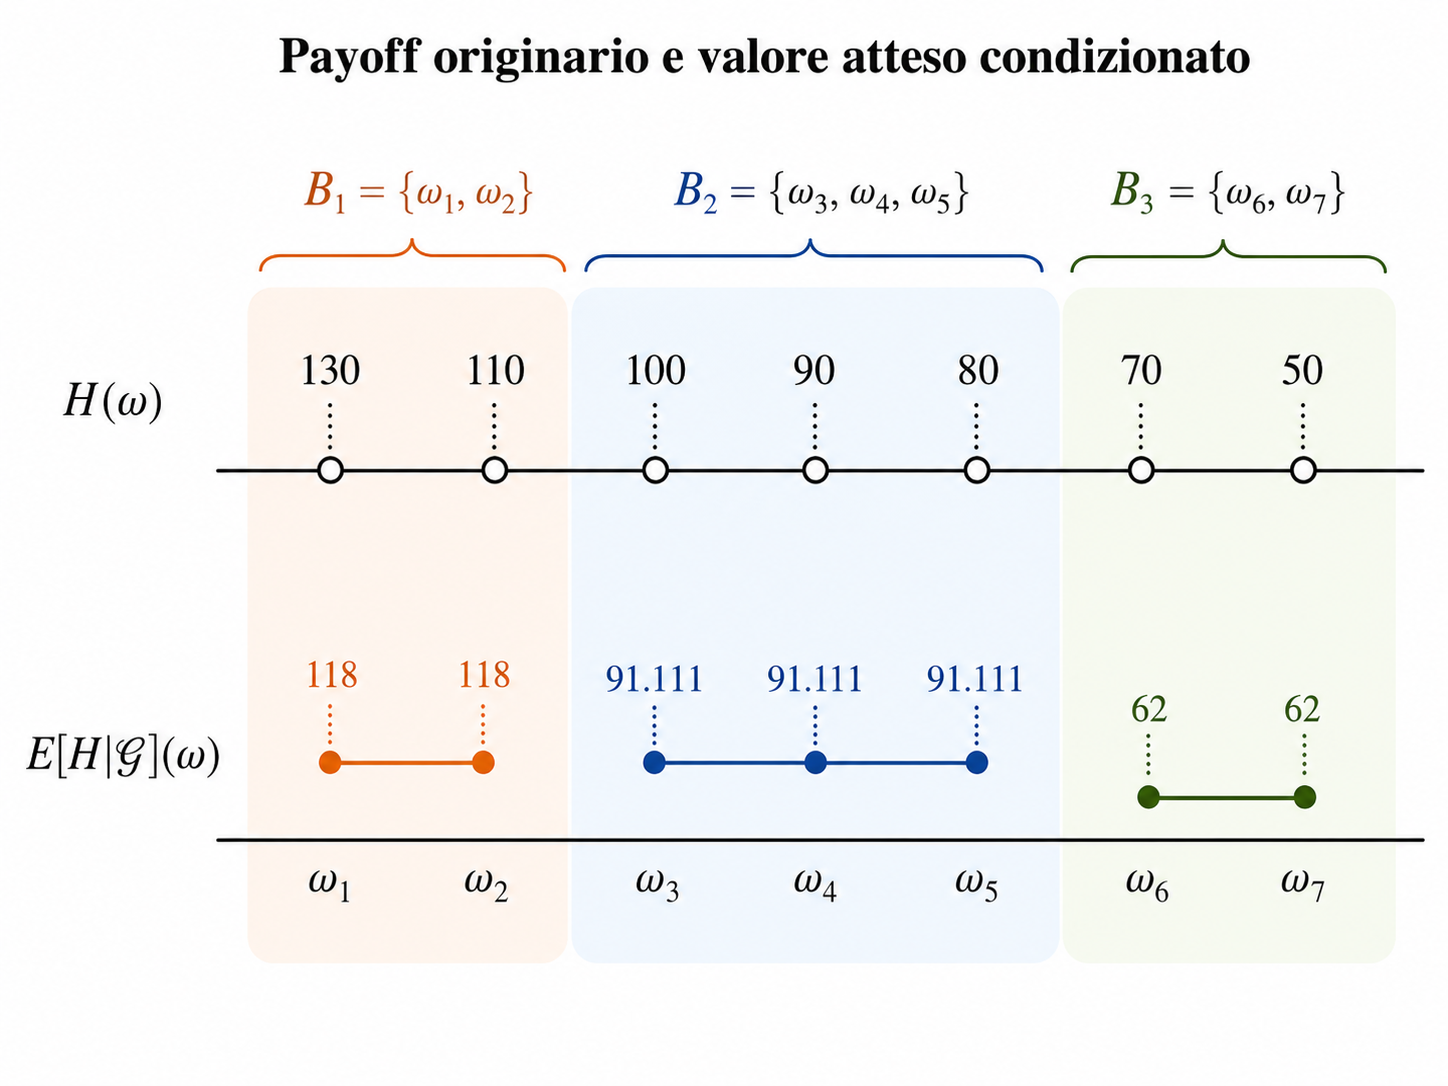
\includegraphics[width=0.76\textwidth,trim=0 60 0 10,clip]{Cap03_Figura_3_3.png}
\end{center}

\vspace{-4mm}

\begin{stepitemize}
\item Il payoff $H$ distingue i sette esiti elementari
$\omega_1,\ldots,\omega_7$.

\item La previsione condizionata $\E[H\mid\G]$ \`{e} invece
\textbf{costante} su ciascun atomo di $\G$.
\end{stepitemize}

%TCIMACRO{\TeXButton{Transition: Box Out}{\transboxout}}%
%BeginExpansion
\transboxout%
%EndExpansion
%TCIMACRO{\TeXButton{EndFrame}{\end{frame}}}%
%BeginExpansion
\end{frame}%
%EndExpansion
%*********************************************

\subsection{Dalla partizione finita alla definizione generale}
%TCIMACRO{\TeXButton{BeginFrame}{\begin{frame}}}%
%BeginExpansion
\begin{frame}%
%EndExpansion

\QTR{frametitle}{Dalla partizione finita alla definizione generale}

%TCIMACRO{\TeXButton{Transparency}{\setbeamercovered{transparent=20}}}%
%BeginExpansion
\setbeamercovered{transparent=20}%
%EndExpansion

Nel caso di una partizione finita, $\G=\sigma(B_1,\ldots,B_n)$, abbiamo
costruito
\[
\E[X\mid\G]
=
\sum_{i=1}^{n}\E[X\mid B_i]\1_{B_i}.
\]

La definizione generale mantiene la stessa idea di
\textbf{coerenza con l'informazione disponibile}. Una variabile casuale $Z$
\`{e} una versione di $\E[X\mid\G]$ se:

\begin{stepenumerate}
\item [1.] $Z$ \`{e} $\G$-misurabile;

\item [2.] per ogni evento $C\in\G$,
\[
\E[Z\1_C]
=
\E[X\1_C].
\]
\end{stepenumerate}

\begin{center}
{\small Il valore atteso condizionato \`{e} definito a meno di uguaglianza
quasi certa.}
\end{center}

%TCIMACRO{\TeXButton{Transition: Box Out}{\transboxout}}%
%BeginExpansion
\transboxout%
%EndExpansion
%TCIMACRO{\TeXButton{EndFrame}{\end{frame}}}%
%BeginExpansion
\end{frame}%
%EndExpansion
%*********************************************

\subsection{Punto di arrivo}
%TCIMACRO{\TeXButton{BeginFrame}{\begin{frame}}}%
%BeginExpansion
\begin{frame}%
%EndExpansion

\QTR{frametitle}{Punto di arrivo: tre valutazioni, due nature}

%TCIMACRO{\TeXButton{Transparency}{\setbeamercovered{transparent=20}}}%
%BeginExpansion
\setbeamercovered{transparent=20}%
%EndExpansion

Sull'esempio a sette scenari:

\begin{center}
{\small
\begin{tabular}{l|c|l}
Informazione & Valutazione & Natura \\ \hline
nessuna & $\E[H]=89.10$ & numero \\
evento $B_1$ osservato & $\E[H\mid B_1]=118$ & numero \\
segnale da osservare, $\G$ &
$118\,\1_{B_1}+91.111\,\1_{B_2}+62\,\1_{B_3}$ & variabile casuale
\end{tabular}
}
\end{center}

\medskip

\begin{stepitemize}
\item Il gradino 2 \`{e} il salto concettuale della lezione: la valutazione
diventa una \textbf{funzione dell'informazione} che sar\`{a} osservata.

\item Restano due domande: perch\'{e} proprio la media? E le valutazioni dei
diversi livelli informativi sono compatibili?
\end{stepitemize}

%TCIMACRO{\TeXButton{Transition: Box Out}{\transboxout}}%
%BeginExpansion
\transboxout%
%EndExpansion
%TCIMACRO{\TeXButton{EndFrame}{\end{frame}}}%
%BeginExpansion
\end{frame}%
%EndExpansion
%*********************************************

%******************
% BLOCCO: Interpretazione: migliore previsione
%******************
\section{Perch\'{e} la media: migliore previsione}

\subsection{Dove siamo: migliore previsione}
%TCIMACRO{\TeXButton{BeginFrame}{\begin{frame}}}%
%BeginExpansion
\begin{frame}%
%EndExpansion

\QTR{frametitle}{Dove siamo: interpretazione}

%TCIMACRO{\TeXButton{Transparency}{\setbeamercovered{transparent=20}}}%
%BeginExpansion
\setbeamercovered{transparent=20}%
%EndExpansion

\begin{center}
{\large Perch\'{e} proprio la media?}
\end{center}

\medskip

\begin{center}
{\footnotesize
\begin{tabular}{c|l|c|l}
Gradino & Informazione & Valutazione & Natura \\ \hline
0 & nessuna & $\E[X]$ & numero \\
1 & un evento $A$ osservato & $\E[X\mid A]$ & numero \\
2 & un segnale da osservare, $\G$ & $\E[X\mid\G]$ & variabile casuale \\
3 & informazione nel tempo, $\F_t$ & $\E[H\mid\F_t]$ & previsione dinamica \\
\end{tabular}
}
\end{center}

\medskip

{\footnotesize
\alert{\textbf{Interpretazione:} $\E[X\mid\G]$ \`{e} la migliore previsione $\G$-misurabile.}

\textbf{Coerenza:} valore atteso totale $\rightarrow$ $\E[\E[X\mid\G]]=\E[X]$ $\rightarrow$ propriet\`{a} della torre.

}

%TCIMACRO{\TeXButton{Transition: Box Out}{\transboxout}}%
%BeginExpansion
\transboxout%
%EndExpansion
%TCIMACRO{\TeXButton{EndFrame}{\end{frame}}}%
%BeginExpansion
\end{frame}%
%EndExpansion
%*********************************************

\subsection{Criterio dell'errore quadratico medio}
%TCIMACRO{\TeXButton{BeginFrame}{\begin{frame}}}%
%BeginExpansion
\begin{frame}%
%EndExpansion

\QTR{frametitle}{$\E[X\mid\G]$ come migliore previsione: il criterio}

%TCIMACRO{\TeXButton{Transparency}{\setbeamercovered{transparent=20}}}%
%BeginExpansion
\setbeamercovered{transparent=20}%
%EndExpansion

\textbf{Problema.} Data l'informazione $\G$, quale variabile casuale
$\G$-misurabile approssima meglio $X$?

\medskip

\textbf{Criterio.} Sia $X$ quadrato-integrabile. Si minimizza l'errore
quadratico medio tra tutte le previsioni ammissibili $Y$:
\[
\min_{Y} \; \E\left[(X - Y)^2\right].
\]

\begin{stepitemize}
\item Una previsione $Y$ \`{e} \textbf{ammissibile} se \`{e}
$\G$-misurabile e quadrato-integrabile: non pu\`{o} usare informazione che
$\G$ non contiene e deve avere errore quadratico medio finito.

\item L'errore quadratico medio misura quanto $Y$ si discosta da $X$
in media, su tutti gli scenari.

\item Il criterio seleziona la previsione che minimizza tale scarto,
rispettando il \textbf{vincolo informativo}.
\end{stepitemize}

%TCIMACRO{\TeXButton{Transition: Box Out}{\transboxout}}%
%BeginExpansion
\transboxout%
%EndExpansion
%TCIMACRO{\TeXButton{EndFrame}{\end{frame}}}%
%BeginExpansion
\end{frame}%
%EndExpansion
%*********************************************

\subsection{La soluzione}
%TCIMACRO{\TeXButton{BeginFrame}{\begin{frame}}}%
%BeginExpansion
\begin{frame}%
%EndExpansion

\QTR{frametitle}{$\E[X\mid\G]$ come migliore previsione: la soluzione}

%TCIMACRO{\TeXButton{Transparency}{\setbeamercovered{transparent=20}}}%
%BeginExpansion
\setbeamercovered{transparent=20}%
%EndExpansion

Se $\G = \sigma(B_1,\ldots,B_n)$, ogni previsione ammissibile deve
essere costante su ciascun atomo $B_i$:
\[
Y = \sum_{i=1}^{n} y_i \1_{B_i}.
\]

\begin{stepitemize}
\item La scelta di $y_i$ \`{e} libera, ma vincolata: tutti gli scenari
in $B_i$ devono ricevere lo stesso valore previsto.

\item La scelta ottima \`{e} la media di $X$ sull'atomo $B_i$:
\[
y_i = \E[X \mid B_i].
\]

\item La previsione ottima coincide quindi con il valore atteso
condizionato rispetto a $\G$:
\[
Y^* = \E[X \mid \G] = \sum_{i=1}^{n} \E[X \mid B_i] \1_{B_i}.
\]
\end{stepitemize}

\begin{center}
{\small $\E[X\mid\G]$ \`{e} la migliore previsione $\G$-misurabile in senso
quadratico, unica quasi certamente.}
\end{center}

%TCIMACRO{\TeXButton{Transition: Box Out}{\transboxout}}%
%BeginExpansion
\transboxout%
%EndExpansion
%TCIMACRO{\TeXButton{EndFrame}{\end{frame}}}%
%BeginExpansion
\end{frame}%
%EndExpansion
%*********************************************

\subsection{Verifica sull'esempio}
%TCIMACRO{\TeXButton{BeginFrame}{\begin{frame}}}%
%BeginExpansion
\begin{frame}%
%EndExpansion

\QTR{frametitle}{Verifica sull'esempio a sette scenari}

%TCIMACRO{\TeXButton{Transparency}{\setbeamercovered{transparent=20}}}%
%BeginExpansion
\setbeamercovered{transparent=20}%
%EndExpansion

Riprendiamo $\G = \sigma(B_1, B_2, B_3)$ e il payoff $H$. Qualsiasi
previsione basata su $\G$ ha la forma:
\[
Y = y_1 \1_{B_1} + y_2 \1_{B_2} + y_3 \1_{B_3}.
\]

\begin{stepitemize}
\item Perch\'{e} $y_1 = 118$? Su $B_1 = \{\omega_1, \omega_2\}$,
con $H(\omega_1) = 130$ e $H(\omega_2) = 110$, qualsiasi altra
costante aumenta l'errore quadratico medio.

\item Analogamente: $y_2 = 91.111$ su $B_2$ e $y_3 = 62$ su $B_3$.

\item La previsione ottima \`{e}:
\[
\E[H\mid\G] = 118\,\1_{B_1} + 91.111\,\1_{B_2} + 62\,\1_{B_3}.
\]
\end{stepitemize}

\textbf{Interpretazione.} $\G$ non distingue $\omega_1$ da $\omega_2$:
la migliore previsione compatibile con $\G$ assegna a entrambi
la media interna all'atomo.

\begin{center}
{\small \textit{Prossimo passo: le valutazioni costruite con informazioni diverse sono compatibili?}}
\end{center}

%TCIMACRO{\TeXButton{Transition: Box Out}{\transboxout}}%
%BeginExpansion
\transboxout%
%EndExpansion
%TCIMACRO{\TeXButton{EndFrame}{\end{frame}}}%
%BeginExpansion
\end{frame}%
%EndExpansion
%*********************************************

%******************
% BLOCCO: Coerenza fra livelli informativi
%******************
\section{Coerenza fra livelli informativi}

\subsection{Dove siamo: coerenza}
%TCIMACRO{\TeXButton{BeginFrame}{\begin{frame}}}%
%BeginExpansion
\begin{frame}%
%EndExpansion

\QTR{frametitle}{Dove siamo: coerenza}

%TCIMACRO{\TeXButton{Transparency}{\setbeamercovered{transparent=20}}}%
%BeginExpansion
\setbeamercovered{transparent=20}%
%EndExpansion

\begin{center}
{\large Le valutazioni dei diversi livelli sono compatibili?}
\end{center}

\medskip

\begin{center}
{\footnotesize
\begin{tabular}{c|l|c|l}
Gradino & Informazione & Valutazione & Natura \\ \hline
0 & nessuna & $\E[X]$ & numero \\
1 & un evento $A$ osservato & $\E[X\mid A]$ & numero \\
2 & un segnale da osservare, $\G$ & $\E[X\mid\G]$ & variabile casuale \\
3 & informazione nel tempo, $\F_t$ & $\E[H\mid\F_t]$ & previsione dinamica \\
\end{tabular}
}
\end{center}

\medskip

{\footnotesize
\textbf{Interpretazione:} $\E[X\mid\G]$ \`{e} la migliore previsione $\G$-misurabile.

\alert{\textbf{Coerenza:} valore atteso totale $\rightarrow$ $\E[\E[X\mid\G]]=\E[X]$ $\rightarrow$ propriet\`{a} della torre.}

}

%TCIMACRO{\TeXButton{Transition: Box Out}{\transboxout}}%
%BeginExpansion
\transboxout%
%EndExpansion
%TCIMACRO{\TeXButton{EndFrame}{\end{frame}}}%
%BeginExpansion
\end{frame}%
%EndExpansion
%*********************************************

\subsection{Regole operative: mappa generale}
%TCIMACRO{\TeXButton{BeginFrame}{\begin{frame}}}%
%BeginExpansion
\begin{frame}%
%EndExpansion

\QTR{frametitle}{Regole operative del valore atteso condizionato}

%TCIMACRO{\TeXButton{Transparency}{\setbeamercovered{transparent=20}}}%
%BeginExpansion
\setbeamercovered{transparent=20}%
%EndExpansion

Per variabili integrabili, il valore atteso condizionato soddisfa alcune
\textbf{regole operative} fondamentali.

\medskip

{\small
\begin{stepenumerate}
\item [1.] \textbf{Linearit\`{a}}:
$\E[aX+bY\mid\G]=a\E[X\mid\G]+b\E[Y\mid\G]$.

\item [2.] \textbf{Estrazione di ci\`{o} che \`{e} noto}: se $Z$ \`{e}
$\G$-misurabile e $ZX$ \`{e} integrabile, allora
$\E[ZX\mid\G]=Z\E[X\mid\G]$.

\item [3.] \textbf{Torre}: se $\G_1\subseteq\G_2\subseteq\F$, allora
$\E\left[\E[X\mid\G_2]\mid\G_1\right]=\E[X\mid\G_1]$.

\item [4.] \textbf{Indipendenza da $\G$}: se $X$ \`{e} indipendente da
$\G$, allora $\E[X\mid\G]=\E[X]$.

\item [5.] \textbf{Indipendenza fra variabili casuali}: se $X$ e $Z$ sono
indipendenti, allora $\E[X\mid Z]=\E[X]$, dove
$\E[X\mid Z]=\E[X\mid\sigma(Z)]$.

\item [6.] \textbf{Jensen condizionata}: se $\psi$ \`{e} convessa,
$\psi\left(\E[X\mid\G]\right)\leq \E[\psi(X)\mid\G]$.
\end{stepenumerate}
}

\begin{center}
{\small La regola 3 \`{e} la forma generale della coerenza fra livelli
informativi.}
\end{center}

%TCIMACRO{\TeXButton{Transition: Box Out}{\transboxout}}%
%BeginExpansion
\transboxout%
%EndExpansion
%TCIMACRO{\TeXButton{EndFrame}{\end{frame}}}%
%BeginExpansion
\end{frame}%
%EndExpansion
%*********************************************

\subsection{La media delle previsioni}
%TCIMACRO{\TeXButton{BeginFrame}{\begin{frame}}}%
%BeginExpansion
\begin{frame}%
%EndExpansion

\QTR{frametitle}{La media delle previsioni restituisce la media ex ante}

%TCIMACRO{\TeXButton{Transparency}{\setbeamercovered{transparent=20}}}%
%BeginExpansion
\setbeamercovered{transparent=20}%
%EndExpansion

\begin{center}
\fbox{\parbox{0.92\textwidth}{
\textbf{Coerenza (2/4) -- media della previsione condizionata.}
\[
\E\left[\E[X\mid\G]\right]=\E[X].
\]
}}
\end{center}

\begin{stepitemize}
\item \`{E} la formula del valore atteso totale scritta con la variabile
casuale $\E[X\mid\G]$.

\item Sull'esempio a sette scenari:
\[
\E\left[\E[H\mid\G]\right]
=118\cdot0.25+91.111\cdot0.45+62\cdot0.30=89.10=\E[H].
\]

\item Prima di osservare il segnale, la previsione media coincide con la
valutazione ex ante: l'informazione \textbf{redistribuisce} la previsione
fra gli stati, ma non ne altera la media.
\end{stepitemize}

%TCIMACRO{\TeXButton{Transition: Box Out}{\transboxout}}%
%BeginExpansion
\transboxout%
%EndExpansion
%TCIMACRO{\TeXButton{EndFrame}{\end{frame}}}%
%BeginExpansion
\end{frame}%
%EndExpansion
%*********************************************

\subsection{Informazione fine e grossolana}
%TCIMACRO{\TeXButton{BeginFrame}{\begin{frame}}}%
%BeginExpansion
\begin{frame}%
%EndExpansion

\QTR{frametitle}{Informazione fine e informazione grossolana}

%TCIMACRO{\TeXButton{Transparency}{\setbeamercovered{transparent=20}}}%
%BeginExpansion
\setbeamercovered{transparent=20}%
%EndExpansion

Sugli stessi sette scenari consideriamo due livelli informativi:
\[
\G_2=\G=\sigma(B_1,B_2,B_3),
\qquad
\G_1=\sigma(B_1\cup B_2,\,B_3).
\]

\begin{stepitemize}
\item $\G_1$ non distingue $B_1$ da $B_2$: i suoi atomi sono
$B_1\cup B_2$ e $B_3$.

\item Ogni evento osservabile con $\G_1$ \`{e} osservabile anche con $\G_2$,
ma non viceversa:
\[
\G_1\subseteq\G_2.
\]

\item $\G_2$ rappresenta un'informazione pi\`{u} \textbf{fine};
$\G_1$ un'informazione pi\`{u} \textbf{grossolana}.
\end{stepitemize}

%TCIMACRO{\TeXButton{Transition: Box Out}{\transboxout}}%
%BeginExpansion
\transboxout%
%EndExpansion
%TCIMACRO{\TeXButton{EndFrame}{\end{frame}}}%
%BeginExpansion
\end{frame}%
%EndExpansion
%*********************************************

\subsection{Con meno informazione}
%TCIMACRO{\TeXButton{BeginFrame}{\begin{frame}}}%
%BeginExpansion
\begin{frame}%
%EndExpansion

\QTR{frametitle}{Con meno informazione: una sola media su $B_1\cup B_2$}

%TCIMACRO{\TeXButton{Transparency}{\setbeamercovered{transparent=20}}}%
%BeginExpansion
\setbeamercovered{transparent=20}%
%EndExpansion

L'evento $B_1\cup B_2$ \`{e} osservabile con $\G_2$, ma non \`{e} un suo
atomo; \`{e} invece un atomo di $\G_1$:
\[
\Prob(B_1\cup B_2)=0.25+0.45=0.70,
\]
\[
\E[H\mid B_1\cup B_2]
=
\frac{\sum_{i=1}^{5}\Prob(\{\omega_i\})H(\omega_i)}{0.70}
=
\frac{70.50}{0.70}
\simeq
100.714.
\]

\begin{stepitemize}
\item La previsione rispetto all'informazione grossolana \`{e}:
\[
\E[H\mid\G_1]=100.714\,\1_{B_1\cup B_2}+62\,\1_{B_3}.
\]

\item $\E[H\mid\G_2]$ mantiene invece separate le previsioni:
$118$ su $B_1$, $91.111$ su $B_2$, $62$ su $B_3$.
\end{stepitemize}

%TCIMACRO{\TeXButton{Transition: Box Out}{\transboxout}}%
%BeginExpansion
\transboxout%
%EndExpansion
%TCIMACRO{\TeXButton{EndFrame}{\end{frame}}}%
%BeginExpansion
\end{frame}%
%EndExpansion
%*********************************************

\subsection{Figura 3.4: informazione fine e grossolana}
%TCIMACRO{\TeXButton{BeginFrame}{\begin{frame}}}%
%BeginExpansion
\begin{frame}%
%EndExpansion

\QTR{frametitle}{Previsione fine e previsione grossolana}

%TCIMACRO{\TeXButton{Transparency}{\setbeamercovered{transparent=20}}}%
%BeginExpansion
\setbeamercovered{transparent=20}%
%EndExpansion

{\centering
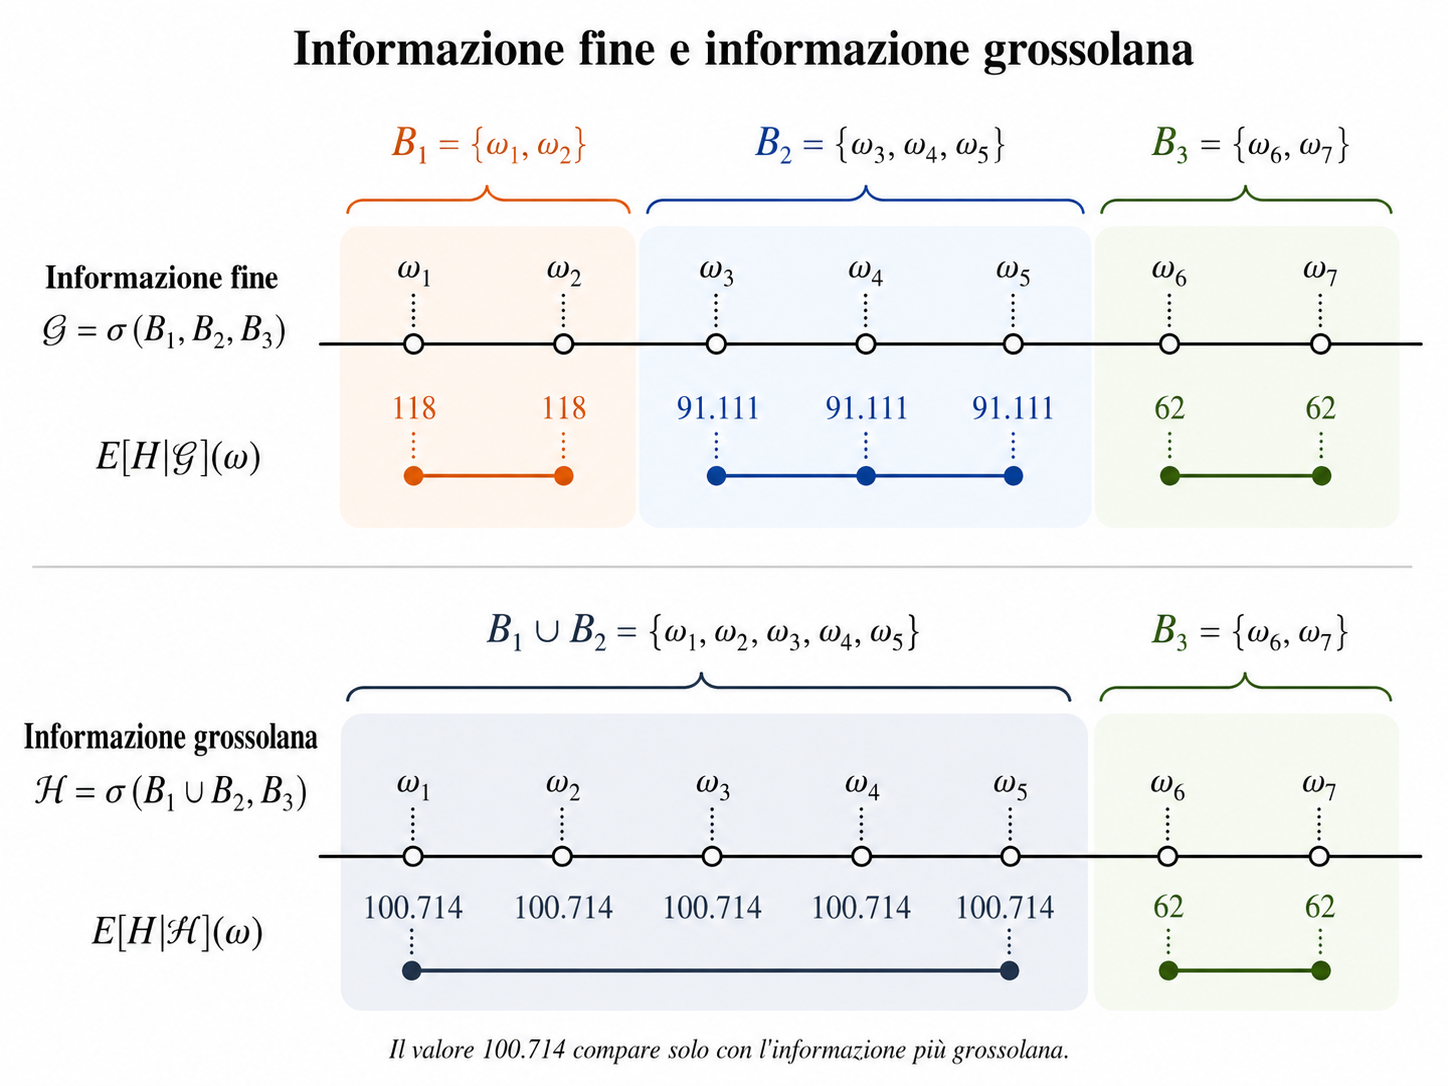
\includegraphics[
  width=0.66\textwidth,
  trim=330 50 0 110,
  clip
]{Cap03_Figura_3_4.png}
\par}

\vspace{-2mm}

{\small In alto: informazione fine $\G_2$ e previsione $\E[H\mid\G_2]$.
In basso: informazione grossolana $\G_1$ e previsione $\E[H\mid\G_1]$,
costante sull'atomo $B_1\cup B_2$.}

%TCIMACRO{\TeXButton{Transition: Box Out}{\transboxout}}%
%BeginExpansion
\transboxout%
%EndExpansion
%TCIMACRO{\TeXButton{EndFrame}{\end{frame}}}%
%BeginExpansion
\end{frame}%
%EndExpansion
%*********************************************

\subsection{Torre: due livelli informativi}
%TCIMACRO{\TeXButton{BeginFrame}{\begin{frame}}}%
%BeginExpansion
\begin{frame}%
%EndExpansion

\QTR{frametitle}{La torre: dalla previsione fine a quella grossolana}

%TCIMACRO{\TeXButton{Transparency}{\setbeamercovered{transparent=20}}}%
%BeginExpansion
\setbeamercovered{transparent=20}%
%EndExpansion

\begin{center}
\fbox{\parbox{0.92\textwidth}{
\textbf{Coerenza (3/4) -- propriet\`{a} della torre.}
Se $\G_1\subseteq\G_2\subseteq\F$:
\[
\E\left[\E[X\mid\G_2]\mid\G_1\right]=\E[X\mid\G_1].
\]
}}
\end{center}

\begin{stepitemize}
\item Sull'atomo $B_1\cup B_2$ di $\G_1$ si fa la media dei valori di
$\E[H\mid\G_2]$:
\[
\frac{118\cdot0.25+91.111\cdot0.45}{0.70}=\frac{70.50}{0.70}\simeq100.714
=\E[H\mid B_1\cup B_2].
\]

\item Sull'atomo $B_3$ il valore resta $62$. Quindi:
\[
\E\left[\E[H\mid\G_2]\mid\G_1\right]
=100.714\,\1_{B_1\cup B_2}+62\,\1_{B_3}
=\E[H\mid\G_1].
\]

\item Con $\G_1=\{\varnothing,\Omega\}$ si ritrova la Coerenza (2/4).
\end{stepitemize}

%TCIMACRO{\TeXButton{Transition: Box Out}{\transboxout}}%
%BeginExpansion
\transboxout%
%EndExpansion
%TCIMACRO{\TeXButton{EndFrame}{\end{frame}}}%
%BeginExpansion
\end{frame}%
%EndExpansion
%*********************************************

%******************
% BLOCCO: Esercizio guidato: gradini 0-2 e coerenza con la perdita L
%******************
\section{Esercizio guidato: la perdita sugli stessi scenari}

\subsection{Testo}
%TCIMACRO{\TeXButton{BeginFrame}{\begin{frame}}}%
%BeginExpansion
\begin{frame}%
%EndExpansion

\QTR{frametitle}{Esercizio guidato: la perdita $L$ sugli stessi scenari}

%TCIMACRO{\TeXButton{Transparency}{\setbeamercovered{transparent=20}}}%
%BeginExpansion
\setbeamercovered{transparent=20}%
%EndExpansion

Un portafoglio pu\`{o} trovarsi negli stessi sette stati di mercato. La perdita
$L$ \`{e} espressa in milioni di euro.

\begin{center}
{\scriptsize
\begin{tabular}{c|l|c|c}
$\omega$ & Stato & $\Prob(\{\omega\})$ & $L(\omega)$ \\
\hline
$\omega_1$ & espansione forte    & 0.10 & 2  \\
$\omega_2$ & espansione moderata & 0.15 & 4  \\
$\omega_3$ & crescita stabile    & 0.15 & 6  \\
$\omega_4$ & stagnazione         & 0.20 & 8  \\
$\omega_5$ & rallentamento       & 0.10 & 12 \\
$\omega_6$ & recessione moderata & 0.18 & 20 \\
$\omega_7$ & recessione severa   & 0.12 & 35 \\
\end{tabular}
}
\end{center}

{\small
\begin{enumerate}
\item Calcolare la perdita media ex ante $\E[L]$.
\item Calcolare $\E[L\mid A]$ per lo scenario di stress
$A=\{\omega_6,\omega_7\}$.
\item Calcolare $\E[L\mid\G]$ con $\G=\sigma(B_1,B_2,B_3)$.
\item Verificare che $\E\left[\E[L\mid\G]\right]=\E[L]$.
\item Calcolare $\E[L\mid\G_1]$ con $\G_1=\sigma(B_1\cup B_2,\,B_3)$.
\end{enumerate}
}

%TCIMACRO{\TeXButton{Transition: Box Out}{\transboxout}}%
%BeginExpansion
\transboxout%
%EndExpansion
%TCIMACRO{\TeXButton{EndFrame}{\end{frame}}}%
%BeginExpansion
\end{frame}%
%EndExpansion
%*********************************************

\subsection{Svolgimento: punti 1-2}
%TCIMACRO{\TeXButton{BeginFrame}{\begin{frame}}}%
%BeginExpansion
\begin{frame}%
%EndExpansion

\QTR{frametitle}{Svolgimento 1-2: perdita media e scenario di stress}

%TCIMACRO{\TeXButton{Transparency}{\setbeamercovered{transparent=20}}}%
%BeginExpansion
\setbeamercovered{transparent=20}%
%EndExpansion

\textbf{Punto 1.} Gradino 0, nessuna informazione:
\[
\E[L] = 0.10\cdot2 + 0.15\cdot4 + \cdots + 0.12\cdot35 = 12.30.
\]

\textbf{Punto 2.} Gradino 1, evento osservato. Lo scenario di stress raccoglie
le due recessioni, con $\Prob(A) = 0.18 + 0.12 = 0.30$:
\[
\E[L \mid A] = \frac{\E[L\,\1_A]}{\Prob(A)}
= \frac{0.18\cdot20 + 0.12\cdot35}{0.30} = \frac{7.80}{0.30} = 26.
\]

\begin{stepitemize}
\item L'informazione di stress pi\`{u} che raddoppia la perdita attesa:
da $12.30$ a $26$.

\item Il payoff $L$ non cambia: cambia la distribuzione con cui viene
valutato.
\end{stepitemize}

%TCIMACRO{\TeXButton{Transition: Box Out}{\transboxout}}%
%BeginExpansion
\transboxout%
%EndExpansion
%TCIMACRO{\TeXButton{EndFrame}{\end{frame}}}%
%BeginExpansion
\end{frame}%
%EndExpansion
%*********************************************

\subsection{Svolgimento: punto 3}
%TCIMACRO{\TeXButton{BeginFrame}{\begin{frame}}}%
%BeginExpansion
\begin{frame}%
%EndExpansion

\QTR{frametitle}{Svolgimento 3: la perdita prevista $\E[L\mid\G]$}

%TCIMACRO{\TeXButton{Transparency}{\setbeamercovered{transparent=20}}}%
%BeginExpansion
\setbeamercovered{transparent=20}%
%EndExpansion

Gradino 2. Le probabilit\`{a} dei blocchi sono $\Prob(B_1)=0.25$,
$\Prob(B_2)=0.45$, $\Prob(B_3)=0.30$.
\[
\E[L\mid B_1] = \frac{0.10\cdot2+0.15\cdot4}{0.25} = 3.20,
\]
\[
\E[L\mid B_2] = \frac{0.15\cdot6+0.20\cdot8+0.10\cdot12}{0.45} = 8.22,
\]
\[
\E[L\mid B_3] = \frac{0.18\cdot20+0.12\cdot35}{0.30} = 26.
\]

Il valore atteso condizionato rispetto a $\G$ \`{e} la variabile casuale:
\[
\E[L\mid\G] = 3.20\,\1_{B_1} + 8.22\,\1_{B_2} + 26\,\1_{B_3}.
\]

%TCIMACRO{\TeXButton{Transition: Box Out}{\transboxout}}%
%BeginExpansion
\transboxout%
%EndExpansion
%TCIMACRO{\TeXButton{EndFrame}{\end{frame}}}%
%BeginExpansion
\end{frame}%
%EndExpansion
%*********************************************

\subsection{Svolgimento: punto 4}
%TCIMACRO{\TeXButton{BeginFrame}{\begin{frame}}}%
%BeginExpansion
\begin{frame}%
%EndExpansion

\QTR{frametitle}{Svolgimento 4: lettura finanziaria e coerenza ex ante}

%TCIMACRO{\TeXButton{Transparency}{\setbeamercovered{transparent=20}}}%
%BeginExpansion
\setbeamercovered{transparent=20}%
%EndExpansion

\begin{center}
{\small
\begin{tabular}{l|c|l}
Informazione & Valore & Interpretazione \\
\hline
Nessuna & $\E[L] = 12.30$ & perdita media ex ante \\
Stato $B_1$ & $\E[L\mid B_1] = 3.20$ & perdita media in espansione \\
Stato $B_2$ & $\E[L\mid B_2] = 8.22$ & perdita media in fase neutra \\
Stato $B_3$ & $\E[L\mid B_3] = 26$ & perdita media in stress \\
\end{tabular}
}
\end{center}

\medskip

Coerenza (2/4) applicata alla perdita:
\[
\E\left[\E[L\mid\G]\right] = 3.20\cdot0.25 + 8.22\cdot0.45 + 26\cdot0.30
= 12.30 = \E[L].
\]

\begin{center}
{\small L'informazione redistribuisce la previsione della perdita fra gli
stati, ma non altera la media ex ante.}
\end{center}

%TCIMACRO{\TeXButton{Transition: Box Out}{\transboxout}}%
%BeginExpansion
\transboxout%
%EndExpansion
%TCIMACRO{\TeXButton{EndFrame}{\end{frame}}}%
%BeginExpansion
\end{frame}%
%EndExpansion
%*********************************************

\subsection{Svolgimento: punto 5}
%TCIMACRO{\TeXButton{BeginFrame}{\begin{frame}}}%
%BeginExpansion
\begin{frame}%
%EndExpansion

\QTR{frametitle}{Svolgimento 5: informazione pi\`{u} grossolana}

%TCIMACRO{\TeXButton{Transparency}{\setbeamercovered{transparent=20}}}%
%BeginExpansion
\setbeamercovered{transparent=20}%
%EndExpansion

Con $\G_1=\sigma(B_1\cup B_2,\,B_3)\subseteq\G$ l'informazione distingue solo
mercato non in stress da mercato in stress; $\Prob(B_1\cup B_2)=0.70$.

\begin{stepitemize}
\item Sull'atomo $B_1\cup B_2$, per la torre si fa la media delle previsioni
fini:
\[
\E[L\mid B_1\cup B_2] = \frac{3.20\cdot0.25 + 8.22\cdot0.45}{0.70}
= \frac{4.50}{0.70} = 6.43.
\]

\item Sull'atomo $B_3$ il valore resta $\E[L\mid B_3]=26$.

\item La previsione rispetto a $\G_1$ \`{e}:
\[
\E[L\mid\G_1] = 6.43\,\1_{B_1\cup B_2} + 26\,\1_{B_3}.
\]

\item Con $\G$ si distinguono tre stati, con $\G_1$ solo due: meno
informazione produce una previsione meno dettagliata.
\end{stepitemize}

\begin{center}
{\small \textit{Prossimo passo: e se l'informazione arriva progressivamente nel tempo?}}
\end{center}

%TCIMACRO{\TeXButton{Transition: Box Out}{\transboxout}}%
%BeginExpansion
\transboxout%
%EndExpansion
%TCIMACRO{\TeXButton{EndFrame}{\end{frame}}}%
%BeginExpansion
\end{frame}%
%EndExpansion
%*********************************************

%******************
% BLOCCO: Gradino 3: l'informazione nel tempo
%******************
\section{Gradino 3: l'informazione nel tempo}

\subsection{Dove siamo: gradino 3}
%TCIMACRO{\TeXButton{BeginFrame}{\begin{frame}}}%
%BeginExpansion
\begin{frame}%
%EndExpansion

\QTR{frametitle}{Dove siamo: gradino 3}

%TCIMACRO{\TeXButton{Transparency}{\setbeamercovered{transparent=20}}}%
%BeginExpansion
\setbeamercovered{transparent=20}%
%EndExpansion

\begin{center}
{\large E se l'informazione arriva nel tempo?}
\end{center}

\medskip

\begin{center}
{\footnotesize
\begin{tabular}{c|l|c|l}
Gradino & Informazione & Valutazione & Natura \\ \hline
0 & nessuna & $\E[X]$ & numero \\
1 & un evento $A$ osservato & $\E[X\mid A]$ & numero \\
2 & un segnale da osservare, $\G$ & $\E[X\mid\G]$ & variabile casuale \\
\alert{3} & \alert{informazione nel tempo, $\F_t$} & \alert{$\E[H\mid\F_t]$} & \alert{previsione dinamica} \\
\end{tabular}
}
\end{center}

\medskip

{\footnotesize
\textbf{Interpretazione:} $\E[X\mid\G]$ \`{e} la migliore previsione $\G$-misurabile.

\textbf{Coerenza:} valore atteso totale $\rightarrow$ $\E[\E[X\mid\G]]=\E[X]$ $\rightarrow$ propriet\`{a} della torre.

}

%TCIMACRO{\TeXButton{Transition: Box Out}{\transboxout}}%
%BeginExpansion
\transboxout%
%EndExpansion
%TCIMACRO{\TeXButton{EndFrame}{\end{frame}}}%
%BeginExpansion
\end{frame}%
%EndExpansion
%*********************************************

\subsection{Dalla sigma-algebra alla filtrazione}
%TCIMACRO{\TeXButton{BeginFrame}{\begin{frame}}}%
%BeginExpansion
\begin{frame}%
%EndExpansion

\QTR{frametitle}{La filtrazione descrive l'informazione che cresce nel tempo}

%TCIMACRO{\TeXButton{Transparency}{\setbeamercovered{transparent=20}}}%
%BeginExpansion
\setbeamercovered{transparent=20}%
%EndExpansion

Finora l'informazione era fissa: una sigma-algebra $\G$ che descriveva un
singolo livello informativo. In finanza l'informazione \`{e} progressiva.

\medskip

La filtrazione \`{e} una successione crescente di sigma-algebre
$\{\F_t\}_{t=0}^{T}$:
\[
\F_0 \subseteq \F_1 \subseteq \cdots \subseteq \F_T \subseteq \F.
\]

\begin{stepitemize}
\item $\F_t$ rappresenta l'informazione disponibile al tempo $t$.

\item L'inclusione $\F_s \subseteq \F_t$ per $s \leq t$ esprime il fatto
che l'informazione non si perde.

\item Sia $H$ un payoff terminale osservato al tempo $T$. La previsione di
$H$ al tempo $t < T$ \`{e} $\E[H\mid\F_t]$.

\item Al crescere di $t$ la previsione diventa pi\`{u} dettagliata. Al tempo
$T$: $\E[H\mid\F_T] = H$.
\end{stepitemize}

%TCIMACRO{\TeXButton{Transition: Box Out}{\transboxout}}%
%BeginExpansion
\transboxout%
%EndExpansion
%TCIMACRO{\TeXButton{EndFrame}{\end{frame}}}%
%BeginExpansion
\end{frame}%
%EndExpansion
%*********************************************

\subsection{Proprieta' della torre in tempo discreto}
%TCIMACRO{\TeXButton{BeginFrame}{\begin{frame}}}%
%BeginExpansion
\begin{frame}%
%EndExpansion

\QTR{frametitle}{La torre nel tempo: previsioni aggiornate e coerenti}

%TCIMACRO{\TeXButton{Transparency}{\setbeamercovered{transparent=20}}}%
%BeginExpansion
\setbeamercovered{transparent=20}%
%EndExpansion

\begin{center}
\fbox{\parbox{0.92\textwidth}{
\textbf{Coerenza (4/4) -- torre nel tempo.}
Se $s \leq t$, allora $\F_s \subseteq \F_t$ e
\[
\E\left[\E[H\mid\F_t]\mid\F_s\right] = \E[H\mid\F_s].
\]
}}
\end{center}

\begin{stepitemize}
\item Prevedere $H$ al tempo $t$ e poi ricondurre quella previsione
all'informazione di $\F_s$ produce la previsione formulata direttamente al
tempo $s$.

\item Le previsioni aggiornate nel tempo sono compatibili con quelle
formulate in precedenza.

\item Con $s=0$ e $\F_0 = \{\varnothing,\Omega\}$:
$\E\left[\E[H\mid\F_t]\right] = \E[H]$.
\end{stepitemize}

\begin{center}
{\small Filtrazione e propriet\`{a} della torre saranno riprese nella
Lezione 5.}
\end{center}

%TCIMACRO{\TeXButton{Transition: Box Out}{\transboxout}}%
%BeginExpansion
\transboxout%
%EndExpansion
%TCIMACRO{\TeXButton{EndFrame}{\end{frame}}}%
%BeginExpansion
\end{frame}%
%EndExpansion
%*********************************************

%******************
% BLOCCO: Esercizio in aula
%******************
\section{Esercizio in aula}

\subsection{Testo}
%TCIMACRO{\TeXButton{BeginFrame}{\begin{frame}}}%
%BeginExpansion
\begin{frame}%
%EndExpansion

\QTR{frametitle}{Esercizio in aula: perdita con distribuzione continua}

%TCIMACRO{\TeXButton{Transparency}{\setbeamercovered{transparent=20}}}%
%BeginExpansion
\setbeamercovered{transparent=20}%
%EndExpansion

Sia $L$ la perdita di un portafoglio su un orizzonte di un periodo. Supponiamo
che $L$ abbia distribuzione uniforme su $[0,20]$:
\[
f_L(\ell) = \frac{1}{20}, \qquad \ell \in [0,20].
\]

Definiamo l'evento di stress come il superamento della soglia $15$:
\[
A = \{L > 15\}, \qquad \Prob(A) = \frac{20-15}{20} = 0.25.
\]

\medskip

\textbf{Domande.}
\begin{enumerate}
\item Calcolare $\E[L]$.
\item Ricavare la densit\`{a} condizionata $f_{L\mid A}(\ell)$.
\item Calcolare $\E[L\mid A]$.
\item Confrontare $\E[L]$ e $\E[L\mid A]$ e interpretare il risultato in
chiave di risk management.
\end{enumerate}

%TCIMACRO{\TeXButton{Transition: Box Out}{\transboxout}}%
%BeginExpansion
\transboxout%
%EndExpansion
%TCIMACRO{\TeXButton{EndFrame}{\end{frame}}}%
%BeginExpansion
\end{frame}%
%EndExpansion
%*********************************************

\subsection{Svolgimento: punti 1-3}
%TCIMACRO{\TeXButton{BeginFrame}{\begin{frame}}}%
%BeginExpansion
\begin{frame}%
%EndExpansion

\QTR{frametitle}{Esercizio: svolgimento (punti 1-3)}

%TCIMACRO{\TeXButton{Transparency}{\setbeamercovered{transparent=20}}}%
%BeginExpansion
\setbeamercovered{transparent=20}%
%EndExpansion

\textbf{Punto 1.} Valore atteso non condizionato:
\[
\E[L] = \int_0^{20} \ell \cdot \frac{1}{20}\,d\ell
= \frac{1}{20}\cdot\frac{\ell^2}{2}\Bigg|_0^{20} = \frac{400}{40} = 10.
\]

\textbf{Punto 2.} La densit\`{a} condizionata si ricava dalla definizione:
\[
f_{L\mid A}(\ell) = \frac{f_L(\ell)}{\Prob(A)} = \frac{1/20}{1/4}
= \frac{1}{5}, \qquad \ell \in (15,20].
\]
La distribuzione condizionata \`{e} uniforme su $(15,20]$.

\medskip

\textbf{Punto 3.} Valore atteso condizionato allo stress:
\[
\E[L\mid A] = \int_{15}^{20} \ell \cdot \frac{1}{5}\,d\ell
= \frac{1}{5}\cdot\frac{\ell^2}{2}\Bigg|_{15}^{20} = \frac{1}{10}(400-225)
= 17.5.
\]

%TCIMACRO{\TeXButton{Transition: Box Out}{\transboxout}}%
%BeginExpansion
\transboxout%
%EndExpansion
%TCIMACRO{\TeXButton{EndFrame}{\end{frame}}}%
%BeginExpansion
\end{frame}%
%EndExpansion
%*********************************************

\subsection{Svolgimento: punto 4}
%TCIMACRO{\TeXButton{BeginFrame}{\begin{frame}}}%
%BeginExpansion
\begin{frame}%
%EndExpansion

\QTR{frametitle}{Esercizio: svolgimento (punto 4)}

%TCIMACRO{\TeXButton{Transparency}{\setbeamercovered{transparent=20}}}%
%BeginExpansion
\setbeamercovered{transparent=20}%
%EndExpansion

\textbf{Punto 4.} Confronto e interpretazione.

\medskip

\begin{center}
\begin{tabular}{l|c|l}
Grandezza & Valore & Significato \\
\hline
$\E[L]$ & $10$ & perdita media su tutti gli scenari \\
$\E[L\mid A]$ & $17.5$ & perdita media negli scenari di stress \\
\end{tabular}
\end{center}

\medskip

\begin{stepitemize}
\item $\E[L] = 10$ considera l'intera distribuzione, compresi gli scenari
favorevoli con perdite basse.

\item $\E[L\mid A] = 17.5$ restringe la valutazione alla coda destra: gli
scenari in cui la perdita supera la soglia $15$.

\item Il condizionamento non modifica la variabile casuale $L$: modifica la
distribuzione con cui viene valutata.

\item La quantit\`{a} $\E[L\mid L>15]=17.5$ misura la perdita media nella
coda destra oltre la soglia $15$. Le misure di rischio di coda saranno
introdotte successivamente.
\end{stepitemize}

%TCIMACRO{\TeXButton{Transition: Box Out}{\transboxout}}%
%BeginExpansion
\transboxout%
%EndExpansion
%TCIMACRO{\TeXButton{EndFrame}{\end{frame}}}%
%BeginExpansion
\end{frame}%
%EndExpansion
%*********************************************

%******************
% BLOCCO: Sintesi
%******************
\section{Sintesi}

\subsection{La scala dell'informazione}
%TCIMACRO{\TeXButton{BeginFrame}{\begin{frame}}}%
%BeginExpansion
\begin{frame}%
%EndExpansion

\QTR{frametitle}{Sintesi: la scala dell'informazione}

%TCIMACRO{\TeXButton{Transparency}{\setbeamercovered{transparent=20}}}%
%BeginExpansion
\setbeamercovered{transparent=20}%
%EndExpansion

\begin{center}
{\footnotesize
\begin{tabular}{c|l|c|l}
Gradino & Informazione & Valutazione & Natura \\ \hline
0 & nessuna & $\E[X]$ & numero \\
1 & un evento $A$ osservato & $\E[X\mid A]$ & numero \\
2 & un segnale da osservare, $\G$ & $\E[X\mid\G]$ & variabile casuale \\
3 & informazione nel tempo, $\F_t$ & $\E[H\mid\F_t]$ & previsione dinamica \\
\end{tabular}
}
\end{center}

\medskip

{\footnotesize
\textbf{Interpretazione:} $\E[X\mid\G]$ \`{e} la migliore previsione $\G$-misurabile.

\textbf{Coerenza:} valore atteso totale $\rightarrow$ $\E[\E[X\mid\G]]=\E[X]$ $\rightarrow$ propriet\`{a} della torre.

}

\medskip

{\small
\begin{stepitemize}
\item Pi\`{u} informazione produce previsioni pi\`{u} dettagliate; la
coerenza fra i gradini \`{e} sempre la stessa idea: valore atteso totale,
$\E[\E[X\mid\G]]=\E[X]$, torre fra $\G_1\subseteq\G_2$, torre fra
$\F_s\subseteq\F_t$.
\end{stepitemize}
}

%TCIMACRO{\TeXButton{Transition: Box Out}{\transboxout}}%
%BeginExpansion
\transboxout%
%EndExpansion
%TCIMACRO{\TeXButton{EndFrame}{\end{frame}}}%
%BeginExpansion
\end{frame}%
%EndExpansion
%*********************************************

\subsection{La lezione in miniatura e gli sviluppi}
%TCIMACRO{\TeXButton{BeginFrame}{\begin{frame}}}%
%BeginExpansion
\begin{frame}%
%EndExpansion

\QTR{frametitle}{Sintesi: la lezione in miniatura e gli sviluppi}

%TCIMACRO{\TeXButton{Transparency}{\setbeamercovered{transparent=20}}}%
%BeginExpansion
\setbeamercovered{transparent=20}%
%EndExpansion

Nell'esempio iniziale a quattro scenari c'era gi\`{a} tutto:
\[
\E[H]=98.25,
\qquad
\E[H\mid\G]=111.25\,\1_{A}+78.75\,\1_{A^c},
\]
\[
98.25=111.25\cdot0.60+78.75\cdot0.40.
\]

\begin{stepitemize}
\item Il valore atteso condizionato non modifica la variabile casuale: modifica
l'informazione rispetto alla quale essa viene valutata.

\item \textbf{Lezione 4.} Questi concetti saranno ripresi in Python mediante
simulazione, distribuzioni empiriche e valori attesi condizionati.

\item \textbf{Lezione 5.} I processi stocastici in tempo discreto saranno
studiati insieme alla filtrazione che li rende adattati: ogni variabile $X_t$
sar\`{a} osservabile rispetto a $\F_t$.
\end{stepitemize}

%TCIMACRO{\TeXButton{Transition: Box Out}{\transboxout}}%
%BeginExpansion
\transboxout%
%EndExpansion
%TCIMACRO{\TeXButton{EndFrame}{\end{frame}}}%
%BeginExpansion
\end{frame}%
%EndExpansion
%*********************************************

\end{document}
